\chapter{Implementation}
% Introducing the Chapter
This chapter gives an overview of the developed musical multi-robot system. The main goal of the implemented system is to allow for a multi-robot (musical) collective to interact with each other in order to achieve emergent and co-ordinating/co-operative behaviour—synchronization specifically in our case—with varying degrees of difficulty and certainty in the environment and communication. More specifically, the goal with the design is to enable the robot collective to achieve so-called \textit{harmonic synchronization} within a relatively short time. What is meant by \textit{harmonic synchronization} will be expounded in Subsection \ref{subsec:harmonic_synchrony}. These goals firstly require of the agents/nodes the modelling of oscillators with their properties, like phase and frequency, as explained further in Subsection \ref{subsec:node}. To allow for interaction and communication between the agents, mechanisms so that the agents can transmit "fire"-signals, as well as listen for other agents's "fire"-signals, is necessary as well, and is presented in Subsection \ref{subsec:fire_signal}.

First, the system and the system components will be presented and introduced. Then, methods implemented for achieving the target goal of \textit{harmonic synchrony} in various synchronization objectives—firstly solely for oscillator-phases, then secondly for both oscillator-phases and oscillator-frequencies—will be described and presented.




% SECTION 1, Introducing the System and the System-components:
\section{The musical multi-robot collective}
\label{sec:developed_system}
\besk{About introduction, overview, and description of the developed system (as well as the system sub-constituents — aka. what the system consists of). $\implies$ in a nutshell: What is the system, and What does it consist of? Why?}

	Envision that we have a multi-agent collective scenario consisting of musical robots modelled as oscillators, solely communicating through brief ``fire''-like audio-signals|greatly inspired by K. Nymoen et al.'s approach for achieving \textit{decentralized harmonic synchronization in mobile music systems} \cite{nymoen_synch}. These agents are initially not synchronized in their firing of audio-signals, but as time goes, they are entraining to synchronize to each other by adjusting their phases and frequencies when or after hearing each other's audio-signals. An illustration of this is given in Figure \ref{fig:initial}.

	% First Intro-illustration figure to easily get a quick idea of what the system/design does/consists of (to be exchanged with a describing system scheme/diagram):
	\begin{figure}[h]
		\centering
			\begin{subfigure}[t]{.5\textwidth}
				\centering\captionsetup{width=.9\linewidth}%
				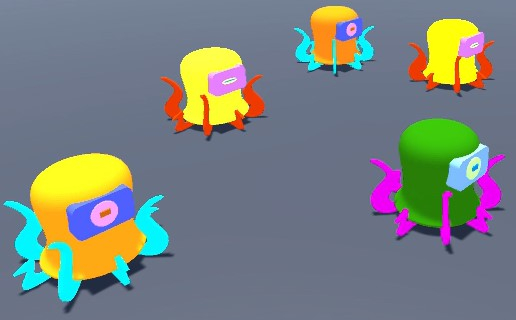
\includegraphics[width=0.9\linewidth]{Assets/Figures/IntroUnsynch.jpg}
				\caption{The agents firing asynchronously at first. Here, only the two Dr. Squiggles with red tentacles are firing simultaneously, but the rest are not.}
				\label{fig:initial:unsynch}
			\end{subfigure}%
			\begin{subfigure}[t]{.5\textwidth}
				\centering\captionsetup{width=.9\linewidth}%
				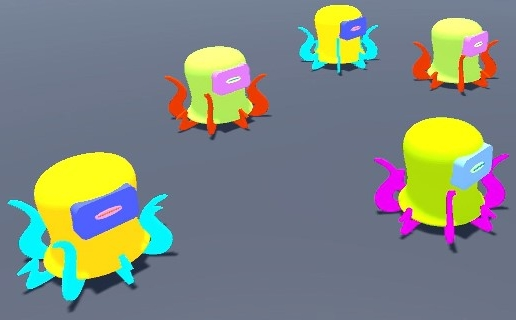
\includegraphics[width=0.9\linewidth]{Assets/Figures/IntroSynch.jpg}
				\caption{Seconds later, after having listened to each other's fire-event signals and adapted themselves accordingly, the agents are here firing synchronously.}
				\label{fig:initial:synch}
			\end{subfigure}
		\caption{Decentralized Synchronization of phases achieved in a musical robot collective, consisting of M. J. Krzyzaniak and RITMO's Dr. Squiggles.}
		\label{fig:initial}
	\end{figure}

	These aforementioned audio-signals to be expounded further in Subsection \ref{subsec:fire_signal}, also referred to as ``fire''-signals, are transmitted whenever an agent's oscillator \textit{peaks} (i.e. after its cycle or period is finished, having phase $\phi(t)=1$)|or actually every second \textit{peak}, due to the target system goal of \textit{harmonic synchrony}. All agents have the ability to listen for such transmitted ``fire''-signals from their neighbours, which they then will use as a trigger to adjust themselves according to some well-designed update-functions to be elaborated upon in Section \ref{sec:phase_methods} and \ref{sec:frequency_methods}.

	% INCLUDE PHASES UNSYNCHED VS. SYNCHED PLOT? See 'Relevant MSc-thesis Concerns'.
		% % Phase-/time-plot Figure with two Subplots. Subplot 1: phase-/time-plot when oscillators are unsynchronized. Subplot 2: phase-/time-plot when oscillators are synchronized
		% \begin{figure}[h]
			% \centering
				% \begin{subfigure}[t]{.5\textwidth}
					% \centering\captionsetup{width=.9\linewidth}%
					% 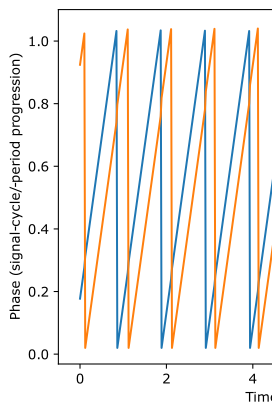
\includegraphics[width=0.9\linewidth]{Assets/Figures/phases_unsynched.png}
					% \caption{Oscillators are initially not (phase-) synchronized.}
					% \label{fig:phases_unsynched}
				% \end{subfigure}%
				% \begin{subfigure}[t]{.5\textwidth}
					% \centering\captionsetup{width=.9\linewidth}%
					% 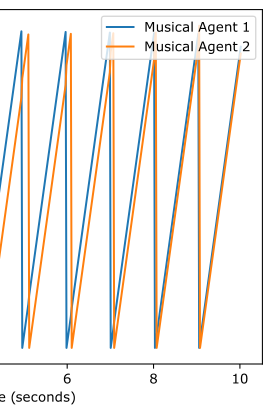
\includegraphics[width=0.9\linewidth]{Assets/Figures/phases_synched.png}
					% \caption{Oscillators are now, seconds later, (phase-) synchronized.}
					% \label{fig:phases_synched}
				% \end{subfigure}
			% \caption{Phase-plots for the agents}
			% \label{fig:initial}
		% \end{figure}



	% Introducing the System Components:
	
	% Om den enkelte noden/agenten med alle egenskaper den har osv.
	\subsection{The Node: the musical robot individual}
	\label{subsec:node}
		\besk{Om den enkelte noden/agenten med alle egenskaper den har osv. (som f.eks. en oscillator-komponent (jf. I.A., III.Intro., og 'Implementation' i Nymoens Firefly-paper))}
		
		Notions like ``agent'', ``node'', ``firefly'', and ``oscillator'' will be used interchangeably throughout the thesis.


	% Om kommunikasjonen til agentene: audio-/``fire''-signalet
	\subsection{Robot communication: the ``fire''-signal}
	\label{subsec:fire_signal}
	
	No individual agent is able to adjust or modify the state of any other agent, and the only means of communication between the agents will be through these ``fire''-signals.
	
		\begin{itemize}
			\item Short and impulsive audio sound/signal, representing a node's phase-climax and ``fire''-/``flash''-event.
			\item Stigmergic co-ordination/communication.
			\item Facilitating PCO (pulse-coupled oscillators), different from phase-coupled oscillators with their differences.
		\end{itemize}

	\gjor{Sjekk oppsummeringen av Nymoen-paperet i Essayet}
	

	% Om target-staten til systemet: harmonisk synkroni
	\subsection{System target state: Harmonic Synchrony}
	\label{subsec:harmonic_synchrony}
		\begin{itemize}
			\item The goal and target state of the system
			\item All agents/nodes having integer-relation frequencies (between each other), so that given a fundamental frequency $\omega_{i,0}$ for the agent $i$ with the lowest frequency in the collective — all other agents have "legal" harmonic frequencies; meaning, all nodes have frequencies in the \tcol{mengde} $\omega_{i,0} \cdot 2^{\mathbb{N}_0}$.
			\item Waveform-Spektrogram av en stemme eller en lyd med Harmonics i seg (f.eks. fra Prariedogs-fyren ellernoe) — som jeg kan sammenlikne med de musikalske nodenes Frekvens-Spektrogram ved siden av. Hvorfor? For å introdusere/presentere/sammenlikne/forklare target-goalet best mulig.
		\end{itemize}
	
	
	
	
	
	
	
	
	
	
	




% SECTION 2, Presenting Methods for Phase-Synchronization:
\section{Synchronizing oscillator-phases}
\label{sec:phase_methods}
\besk{About various methods/algorithms/approaches (the nitty gritty) implemented to achieve the target/goal state(s). $\implies$ in a nutshell: What different but comparable methods did you use to achieve your goal(s) for Phase-Synchronization?}

	If we first assume constant and equal oscillator-frequencies in our agents, we can take a look at how the agents adjust their|initially random|phases in order to synchronize to each other. This is then in contrast to the case in Section \ref{sec:frequency_methods} where heterogenous and randomly initialized oscillator-frequencies in the musical agents are used and synchronized.
	
	The goal state of the agents is for now to fire/flash simultaneously, after having started firing/flashing at random initially. Note that this is a different goal from the final and ultimate goal of \textit{harmonic synchrony}. This is actually not true — as firing/flashing simultaneously technically would be considered having achieved harmonic synchrony. Hence, this "sub-goal" is actually a sufficient and weaker goal w.r.t. the main goal of harmonic synchrony.
	
	In order for the musical agents to synchronize to each other, they will have to—due to their heterogenous and randomly initialized phases—adjust or update their own phases according to some well-designed update-/adjustment-functions, as presented below.
	
	When it comes to the temporality and timing of when these updating functions are used and applied; Musical agents's phases get updated/adjusted immediately as ``fire''-/``flash''-events from neighbouring robots are perceived.

	
	
	% Mirollo-Strogatz's Phase-Synchronization
	\subsection{Mirollo-Strogatz's ``Standard'' Phase-adjustment}
	
	One approach having been used to achieve this in the past is Mirollo-Strogatz's ``Standard'' Phase-adjustment in oscillators \cite{mirollo_strogatz_PCO_synch}, as illustrated in Figure \ref{fig:strog_phase}.
			
	\begin{figure}[h]
		\centering
		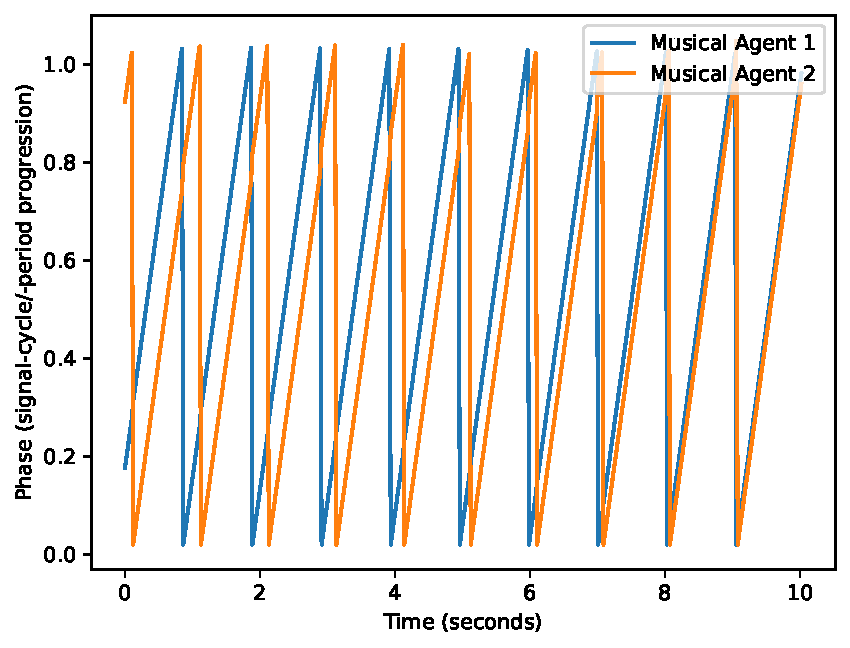
\includegraphics[width=0.9\linewidth]{Assets/Figures/MirolloStrogatzPhaseAdjustment.pdf}
		\caption{``Standard'' Phase-Adjustment with Mirrollo-Strogatz's approach}
		\label{fig:strog_phase}
	\end{figure}
	
	Each musical node gets a new phase, $\phi(t^+) = P(\phi(t))$, accoring to the \textbf{phase update function \eqref{strog_phase}} upon perceiving a ``fire''-event from one of the other musical nodes:
	
	\begin{equation}\label{strog_phase}
	P(\phi(t)) = (1 + \alpha)\phi(t)	,
	\end{equation}
	
	where ``\textit{$\alpha$ is the pulse coupling constant, denoting the strength between nodes}'' \cite{nymoen_synch}, and $t^+$ denotes the time-step immediately after phase-climax. So, if $\alpha = 0.1$ e.g., then a musical node's new and updated phase, immediately after hearing a ``fire''-signal from another node, will be equal to $\phi(t^+) = P(\phi) = (1 + 0.1)\phi = 1.1\phi$. 110\% of its old phase $\phi$, that is. Hence, and in this way, the node would be ``pushed'' to fire sooner than it would otherwise (as nodes fire once they have reached phase-climax $\phi=1$).
		
	
	
	
	% K. Nymoen's Phase-Synchronization
	\subsection{K. Nymoen's Bi-Directional Phase Shifts}
	
	\begin{figure}[h]
		\centering
		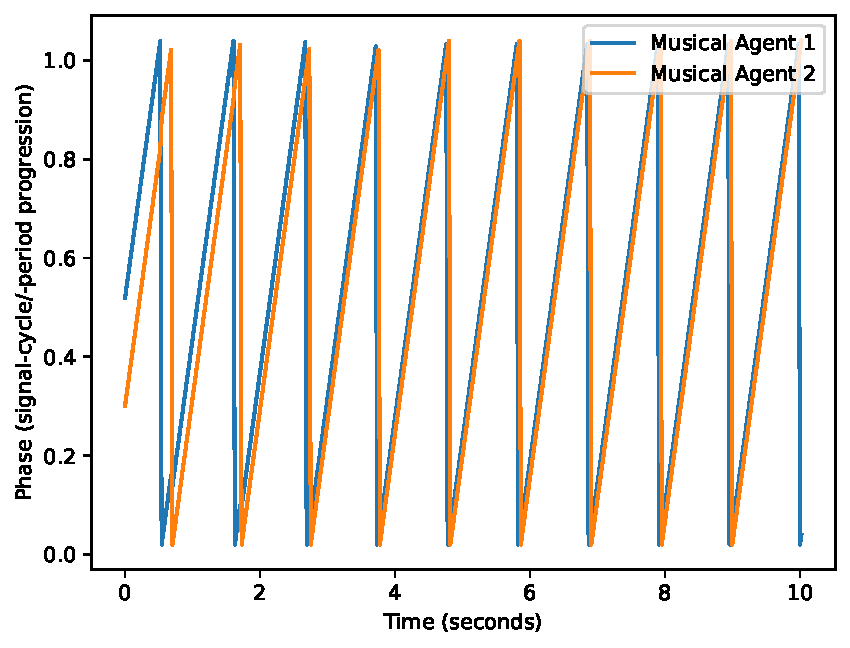
\includegraphics[width=0.9\linewidth]{Assets/Figures/NymoenPhaseAdjustment.pdf}
		\caption{Bi-directional Phase-Adjustment with K. Nymoen et al.'s approach}
		\label{fig:nymoen_phase}
	\end{figure}
	
	This Phase-adjustment, as in Figure \ref{fig:nymoen_phase}, works very similarly to the Phase-adjustment performed in the ``standard'' \textbf{\textit{Mirollo-Strogatz}} approach presented earlier; the only difference being that now, nodes update their phases with the slightly more complex \textbf{phase update function \eqref{nymoen_phase}} when hearing a ``fire''-event from one of the other musical nodes — allowing for both larger, but also smaller, updated phases:
	
	\begin{equation}
	\label{nymoen_phase}
		P(\phi) = \phi - \alpha \cdot sin(2\pi\phi) \cdot | sin(2\pi\phi) |
	\end{equation}
	
	The fact that new and updated phases can both be larger, but also smaller, compared to the old phases, is exactly what's meant by the Phase-adjustment being \textbf{\textit{Bi-Directional}}, or as the authors call it in the paper as using ``\textit{both excitatory and inhibitory phase couplings between oscillators}'' \cite{nymoen_synch}.
	
	The effects then of adjusting phases—upon hearing ``fire''-events, according to this newest update-function \eqref{nymoen_phase}—are that the nodes's phases now get decreased if $\phi(t)$ is lower than 0.5, increased if $\phi(t)$ is higher than 0.5, and neither—at least almost—if the phases are close to $0.5$. This is due to the negative and positive sign of the sinewave-component in Equation \eqref{nymoen_phase}, as well as the last attenuating factor in it of $| sin(2\pi\phi) | \approx | sin(2\pi \frac{1}{2}) | = | sin(\pi) | = | 0 | = 0$, then if we have $\phi(t) \approx 0.5 = \frac{1}{2}$.

	
	
	
	
	
	










	

% SECTION 3, Presenting Methods for Phase- & Frequency-Synchronization:
\section{Synchronizing both oscillator -phases and -frequencies}
\label{sec:frequency_methods}
\besk{About various methods/algorithms/approaches (the nitty gritty) implemented to achieve the target/goal state(s). $\implies$ in a nutshell: What different but comparable methods did you use to achieve your goal(s) for Frequency- \& Phase-Synchronization?}

	% Om Update-functions for frekvens-oppdateringene
	Now over to the slightly more complex issue of adjusting and synchronizing frequencies—as well as phases—in the agent-/oscillator-collective. We introduce randomly initialized, non-constant, and heterogenous oscillator-frequencies in our musical agents — allowing in the music collective the playing of rhythmic patterns like \tcol{doubles, fourths, eights (FRA NYMOEN: subdivisions of a measure, i.e. quarter notes and 8ths. "Temporal components in music tend to appear in an integer-ratio relation to each other (e.g., beats, measures, phrases, or quarter notes, 8ths, 16ths)")} etc. The agents are now then required to not only synchronize their phases to each other, but now also their initially different and random frequencies — so that frequencies are ``legal'' and \textit{harmonically synchronized}.
	
	The goal state now will not be exactly equal frequencies and phases, but rather the goal state of \textit{harmonic synchrony}.
	
	In order for the musical agents to synchronize to each other, they will have to adjust or update their own phases and frequencies according to some well-designed update-/adjustment-functions. Three approaches/methods that was implemented to achieve this, and the goal state of \textit{harmonic synchrony}, is presented now. Notice the increasing degree of \textit{Computational Self-Awareness} endowed/utilized/included in the methods.
	
	
	
	
	% FREQ.-SYNCH APPROACH 1: LOW LEVEL Self-Awareness
	% Person X's "simpler" Frequency-Synchronization without any Self-Awareness components
	\subsection{Person X's low SA-level frequency-updates}
	
	A simpler strategy/method for achieving Harmonic Synchronization including Frequeny-Adjustment, specifically with no Self-Awareness capabilities, if it exists.
	
	
	

	
	% FREQ.-SYNCH APPROACH 2: MID LEVEL Self-Awareness
	% K. Nymoen's Frequency-Synchronization with some Self-Awareness (which as far as I know only works together with K. Nymoen's Phase-Synchronization)
	\subsection{K. Nymoen's mid SA-level frequency-updates}
	
	This approach to Frequency Adjustment stands in contrast to previous approaches to synchronization in oscillators \tcol{cite(fixed\_freqs, fixed\_range\_freqs)} where the oscillators's frequencies are either equal and fixed, or where frequencies are bound to initialize and stay within a fixed interval/range.
	
	In order to achieve this goal of \textit{harmonic synchrony} in conjunction with|or rather through|frequency adjustment, we have to go through a few steps to build a sophisticated enough update-function able to help us achieve this.
	
	When it comes to the temporality and timing of when these update functions are used and applied; Musical agents's phases get updated/adjusted immediately as ``fire''-/``flash''-events are perceived, whereas agents's frequencies do not get updated until the end of their oscillator-cycle (i.e. when having a phase-climax $\phi(t)=1$). This is also the reason why frequencies are updated discretely, not continuously. So-called H-values however, being ``contributions'' with which the frequencies are to be updated according to, are immediately calculated and accumulated when agents are perceiving a ``fire''-/``flash''-event — and then finally used for frequency-adjustment/-updating at phase-climaxes.
			
	Each agent $i$ update their frequency, on their own phase-climax (i.e. when $\phi_i(t)=1$), according to the frequency-update function $\omega_i(t^+)$:
	
	\begin{equation}
		\omega_i(t^+) = \omega_i(t) \cdot 2^{F(n)},
	\end{equation}
	
	where $t^+$ denotes the time-step immediately after phase-climax, $\omega_i(t)$ is the old frequency of the agent at time $t$, and $F(n) \in [-1,1]$ is a quantity denoting how much and in which direction a node should update its frequency after having received its $n$th ``fire''-signal.
	
	This is how we obtain the aforementioned $F(n)$-quantity:
	
	
	% Om epsilon(n):
	\subsubsection{Step 1: the ``in/out-of synch'' error-measurement/-score, $\epsilon(\phi(t))$}
	
	Describing the error measurements at the n-th ``fire''-event, we introduce an Error Measurement function.
	
	The Error Measurement function \eqref{error_measurement}, plotted in Figure \ref{fig:error_measurement}, is calculated immediately by each agent $i$, having phase $\phi_i(t)$, when a ``fire''-event signal from another agent is detected by agent $i$ at time $t$.
	
	\begin{equation}
	\label{error_measurement}
		\epsilon(\phi_i(t)) = sin^2(\pi\phi_i(t))
	\end{equation} \nl
	
	\begin{figure}[h!]
		\centering
		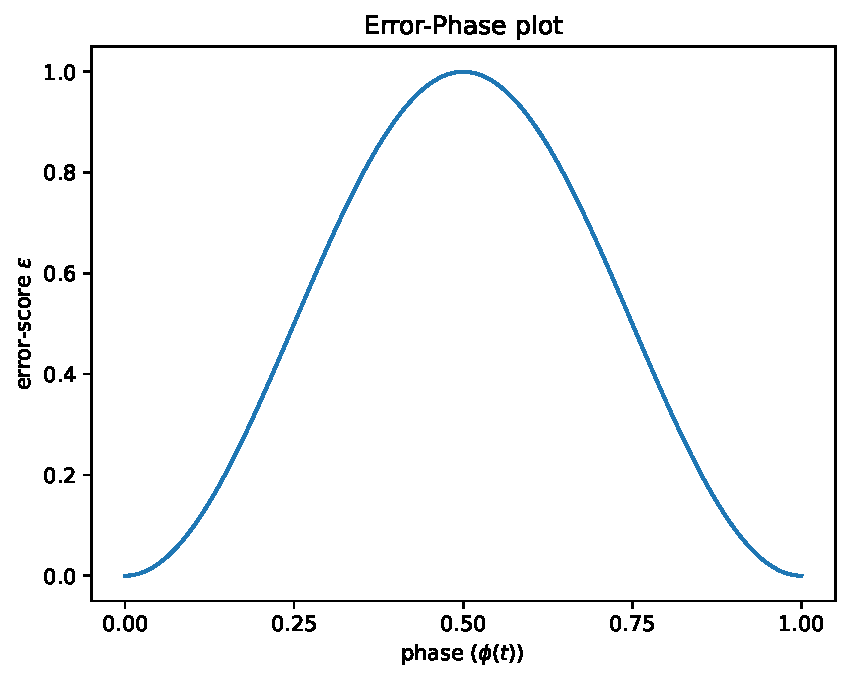
\includegraphics[width=0.8\linewidth]{Assets/Figures/PhaseErrorFunction.pdf}
		\caption{Error Measurement \eqref{error_measurement} plotted as a function of Phase}
		\label{fig:error_measurement}
	\end{figure}
	
	As we can see from this Error-Function, the error-score is close to 0 when the agent's phase $\phi_i(t)$ is itself close to 0 or 1 (i.e. the agent either just fired/flashed, or is about to fire/flash very soon). The error-score is the largest when an agent perceives a ``fire''-signal while being half-way through its own phase (i.e. having phase $\phi(t)=0.5$). We could also then ask ourselves, does not this go against the main/target goal of the system, being \textit{harmonic synchrony} — if agents are allowed to be ``half as fast'' as each other? 
	
	We could imagine a completely ``legal'' and harmonically synchronous scenario where two agents have half and double the frequency of each other. The agent with half the frequency of the faster agent would then have phase $\phi(t)=0.5$ when it would hear the faster agent ``fire''/``flash'' — leading to its Error-score $\epsilon(0.5) = sin^2(\pi/2) = 1$, which then makes it seem like the slower agent is maximally out of synch, when it is actually perfectly and harmonically synchronized. \tcol{???} \inkl{This calls out for an attenuating mechanism in our frequency update function, in order to ``cancel out'' this contribution so that perfectly harmonically synchronized agents will not be adjusted further despite their high Error-measurement.}
	
	This Error-Measurement/-Score forms the basis and fundament for the first component of Self-awareness, being the \textit{self-assessed synchrony-score} $s(n)$.
	
	% Om s(n):
	\subsubsection{Step 2: The first self-awareness component, s(n)}
	This aforementioned self-assessed synchrony-score, $s(n)$, is in fact simply the median of a list \tcol{(was originally in K. Nymoen et al.'s approach a running median filter over the discrete error measurement function)} containing \textit{m} Error-scores $\epsilon$. Such a list is easily implemented in C\# by declaring a List$<$float$>$ called \textit{errorBuffer} e.g. (i.e. \textit{errorBuffer} is a list containing floating point values):
	
	\begin{equation}
	\label{error_buffer}
		errorBuffer = \{\epsilon(n), \epsilon(n-1), ... , \epsilon(n-m)\},
	\end{equation} \nl
	
	then leading to:
	
	\begin{equation}
	\label{self_assessed_synch}
		\begin{array}{rrclcl}
		s(n) & = & median(errorBuffer) \\ 
		& = & median(\{\epsilon(n), \epsilon(n-1), ... , \epsilon(n-m)\}) \in [0, 1],
		\end{array}
	\end{equation} \nl
	
	where $n$ is the latest observed ``fire-event'', and $m$ is the number of the last observed ``fire''-events we would like to take into account when calculating the self-assessed synch-score.
	
	If we then have a high $s(n)$-score, it tells us that the median of the $k$ last error-scores is high, or in other words that we have mainly high error-scores — indicating that this agent is out of synch. Conversely, if we have a low $s(n)$-score, indicating mainly low error-scores for the agent — then we have an indication that the agent is in synch, hence leading to low error scores, and in turn low $s(n)$-scores. 
	
	In other words, we then have a way for each agent to assess themselves how much in or out of synch they believe they are compared to the rest of the agents. This is then the first degree/aspect of \tcol{(public?)} Self-awareness in the design.
	
	% Om rho(n):
	\subsubsection{Step 3: frequency update amplitude- \& sign-factor, $\rho(n)$}
	
	Describing the amplitude and sign of the frequency-modification of the n-th ``fire-event'' received. It is used to say something about in which direction, and in how much, the frequency should be adjusted.
	
	\begin{equation}
	\label{amp_sign_freq_adj}
		\rho(\phi) = - sin(2\pi\phi(t)) \in [-1, 1]
	\end{equation}
	
	For example, if a node $i$ has phase $\phi_i(t)=1/4$, it gets a value $\rho(1/4) = - sin(\pi/2) = -1$; meaning, the node's frequency should be decreased (with the highest amplitude actually) in order to "slow down" to wait for the other nodes. Conversely, if a node $j$ has phase $\phi_j(t)=3/4$, it gets a value $\rho(3/4) = - sin(3/2 \pi) = -(-1) = 1$; meaning, the node's frequency should be increased (with the highest amplitude) in order to getting "pushed forward" to catch up with the other nodes.
	
	Acts as an attenuating factor, when $\phi(t)\approx0.5$, in the making of the H-value — supporting the goal of \textit{harmonic synchrony}.

	% Om H(n)-verdiene:
	\subsubsection{Step 4: the H-value, and the H(n)-list}
	
	The following value, being ``frequency-update-contributions'', is then (as previously mentioned) calculated immediately when the agent perceives another agent's ``flashing''-signal:
	
	\begin{equation}
	\label{h_value}
		H(n) = \rho(n) \cdot s(n)
	\end{equation}
	
	Here we then multiply a factor $\rho(n)$ representing how much, as well as in which direction, the node should adjust its frequency, together with a factor $s(n) \in [0,1]$ of the adjusting node's self-assessed synch-score. To recall, the self-assessed synch-score $s(n)$ tells an adjusting node how in- or out-of-synch it was during the last $m$ perceived ``fire''-/``flash''-events — where $s(n)=0$ signifies a mean of 0 in error-scores, and $s(n)=1$ signifies a mean of 1 in error-scores. So then if this $H$-value is to be used to adjust the nodes's frequencies with, the frequency will then be adjusted in a certain direction and amount (specified by $\rho(n)$) — given that the node is \textit{enough} ``out of synch''/``unsynchronized'' (in the case $s(n)$ is considerably larger than 0).
	
	The H-value says something about how much ``out of phase'' the node was at the time the node's $n$th ``flashing''-signal was perceived (and then followingly how much it should be adjusted, as well as in which direction after having been multiplied together with a sign-factor $\rho(n))$, given then that this H-value also consists of the \textit{self-assessed synch score s(n)} — which again simply was the median of the list of error-scores, \textit{errorBuffer} in our case.
	
	We could look at this $H$-value as representing the direction and amplitude of the frequency adjustment weighted by the need to adjust (due to being out of synch) at the time of hearing ``fire''-/``flash''-event $n$. Or in other words, this $H$-value is then the $n$-th contribution with which we want to adjust our frequency with.
	
	Especially interesting cases are when we have $\phi(n)\approx0.5 \implies \rho(n)\approx\pm0$, as well as the last $m$ Error-scores $\epsilon(n)$ being close to 0, also leading to $s(n)\approx0$. In both of these two cases the entire frequency-adjustment contribution $H$ would be cancelled out, due to harmonic synchronization (legally hearing a ``fire''-/``flash''-event half-way through ones own phase) in the first case, and due to not being out of synch in the latter (having low Error-Measurements). Cancelling out the frequency adjustment contribution in these cases is then not something bad, but something wanted and something that makes sense. If these $H$-values then are cancelled out or very small, it is indicative of that nodes are already in \textit{harmonic synchrony}, and hence should not be ``adjusted away'' from this goal state. On the other side, if these $H$-values then are different (e.g. closer to -1 and 1), it is indicative of that nodes are not yet in \textit{harmonic synchrony}, and that they hence should be ``adjusted closer'' to the goal state.
	
	All the calculated H-values are in my implementation accumulated and stored in an initially empty C\#-list (of floats), referred to as $H(n)$, at once they are calculated. The $H(n)$-list is then consecutively ``cleared out'' or ``flushed'' when its H-values have been used for the current cycle/period's frequency adjustment (i.e. at the phase climax, when $\phi(t)=1$), and is then ready to accumulate new H-values during the next cycle/period.
	
	% Om F(n) og selve oppdateringen av frekvens:
	\subsubsection{The final step: the frequency update function, $\omega_i(t^+)$}
	
	Putting it all together.
	
	When an agent $i$ then has a phase-climax ($\phi_i(t)=1$), it updates its frequency to the new $\omega_i(t^+)$ accordingly:
	
	\begin{equation}
	\label{freq_adj}
		\omega_i(t^+) = \omega_i(t) \cdot 2^{F(n)},
	\end{equation}
	
	where $t^+$ denotes the time-step immediately after phase-climax, and $F(n)$ is found by:
	
	\begin{equation}
	\label{f_value}
		F(n) = \beta\sum_{x=0}^{k-1}\frac{H(n-k)}{k},
	\end{equation}
	
	where $\beta$ is the frequency coupling constant, $k$ is the number of heard/received ``fire-event''s from the start of the last cycle/period to the end (i.e. the phase-climax, or \textit{now}) — and the rest of the values are as described above.
	
	This $F(n)$-value then, as we see in Equation \eqref{f_value}, is a weighted average of all the node's $H(n)$-values accumulated throughout the node's last cycle.
	
	
	
	
	
	% FREQ.-SYNCH APPROACH 3: HIGH LEVEL Self-Awareness
	% Hopefully an improved method with some additional Self-Awareness components
	\subsection{Thorvaldsen's high SA-level frequency-updates}
	
	My new proposed algorithm for achieving Harmonic Synchronization including Frequeny-Adjustment, comprising several additional Self-Awareness components compared to K. Nymoen's approach (jf. \textbf{Thorvaldsen's improved approach} på reMarkablen). I want to best Nymoen.